\documentclass[12pt,compress,ngerman,utf8]{beamer}
\usepackage[ngerman]{babel}
\usepackage{ragged2e}
\usepackage{wasysym}
\usepackage[protrusion=true,expansion=true]{microtype}

\titlegraphic{\leavevmode\smash{\raisebox{6cm}{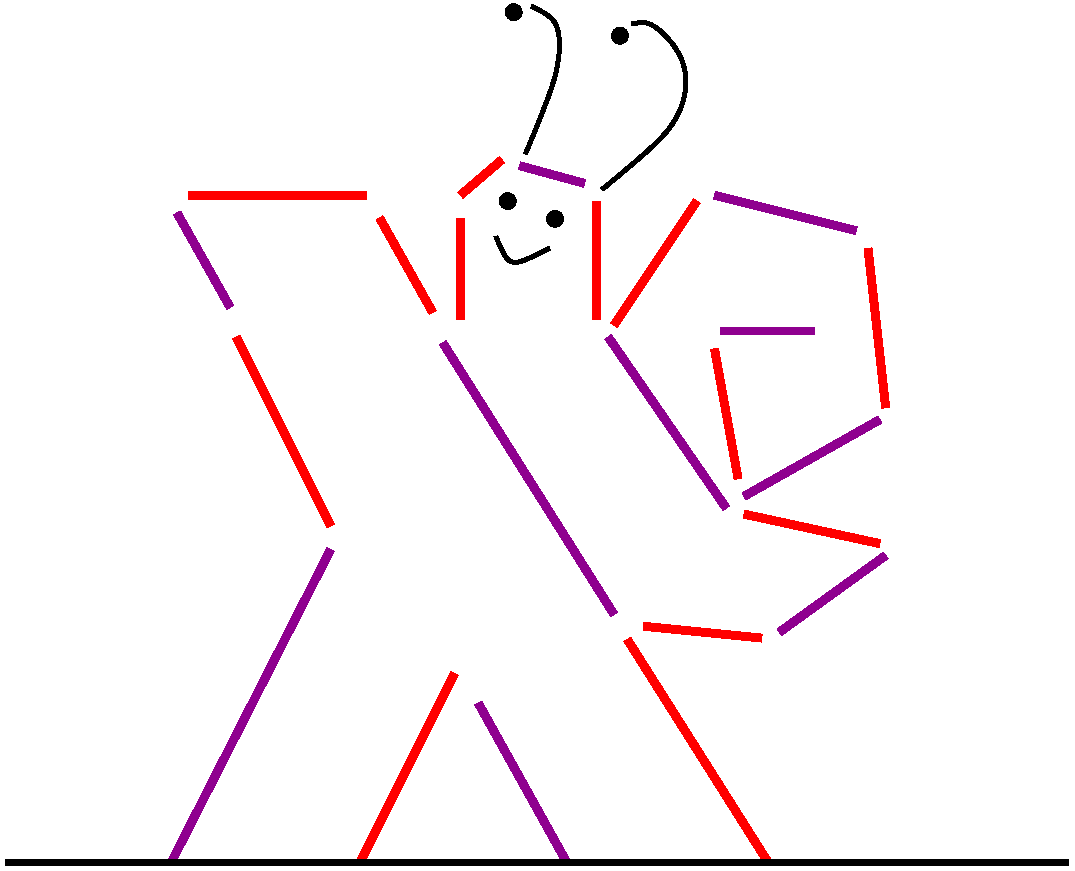
\includegraphics[scale=0.25]{images/lambdaschnecke}}}}
\title{\smiley{} Kombinatorische Spieltheorie \smiley{} \\ mit surrealen Zahlen und Haskell}
\author[Augsburger Curry Club]{
    Ingo Blechschmidt \\[0.1em] \scriptsize\texttt{<iblech@speicherleck.de>}
}
\date[2016-02-25]{\vspace*{-2.5em}\\\scriptsize Augsburger Curry-Club \\ 25.
Februar 2016}

\usetheme{Warsaw}

\useinnertheme{rectangles}

\usecolortheme{seahorse}
\definecolor{mypurple}{RGB}{150,0,255}
\setbeamercolor{structure}{fg=mypurple}

\usefonttheme{serif}
\usepackage[T1]{fontenc}
\usepackage{libertine}

\setbeamertemplate{navigation symbols}{}
\setbeamertemplate{headline}{}
\setbeamertemplate{footline}{}

\setbeamertemplate{title page}[default][colsep=-1bp,rounded=false,shadow=false]
\setbeamertemplate{frametitle}[default][colsep=-2bp,rounded=false,shadow=false,center]

\setbeamertemplate{frametitle}{%
  \vskip1em%
  \leavevmode%
  \begin{beamercolorbox}[dp=1ex,center]{}%
      \usebeamercolor[fg]{item}{\textbf{\textsf{\Large \insertframetitle}}}
  \end{beamercolorbox}%
}

\begin{document}

\frame{\vspace*{10em}\titlepage}

\frame[plain]{\footnotesize\justifying
  \begin{itemize}\justifying
    \item In der kombinatorischen Spieltheorie untersucht man
    Zwei-Personen-Spiele ohne Zufallselemente und ohne verborgene Information.
    Verlierer ist, wer keinen Zug mehr tätigen kann.
    \item Jeder Spielsituation eines solchen Spiels ordnet man einen Wert zu.
    \item Ist dieser positiv, besitzt der linke Spieler eine Gewinnstrategie.
    Ist er negativ, besitzt der rechte eine. Ist er Null, so besitzt der als
    zweites ziehende Spieler eine Gewinnstrategie. Und ist er "`fuzzy zu
    Null"', so besitzt der als erstes ziehende Spieler eine Gewinnstrategie.
    \item Die Werte sind nicht gewöhnliche reelle Zahlen, sondern
    \emph{surreale Zahlen} oder etwas allgemeiner \emph{Games}.
    \item Es gilt ein wichtiges Kompositionalitätsprinzip: Zerfällt eine Spielsituation
    in zwei unabhängige Teile, so ist der Gesamtwert die Summe der Einzelwerte.
    \item Mögliche Werte sind vertraute Zahlen wie~$0$, $1$, $-1$
    und~$\frac{3}{4}$; aber auch Zahlen wie~$1/\omega$ und~$\omega - 1$. Dabei
    ist~$\omega$ eine vornehme Schreibweise für die "`einfache unendlich große
    Zahl"', die es im Bereich der surrealen Zahlen gibt.
  \end{itemize}
}

\frame[plain]{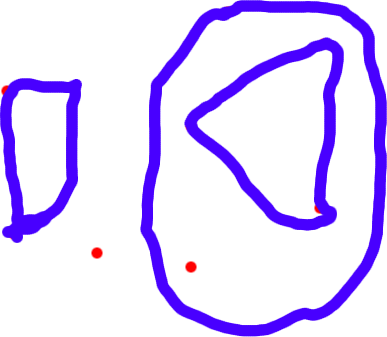
\includegraphics[width=\textwidth]{images/surreal1}}
\frame[plain]{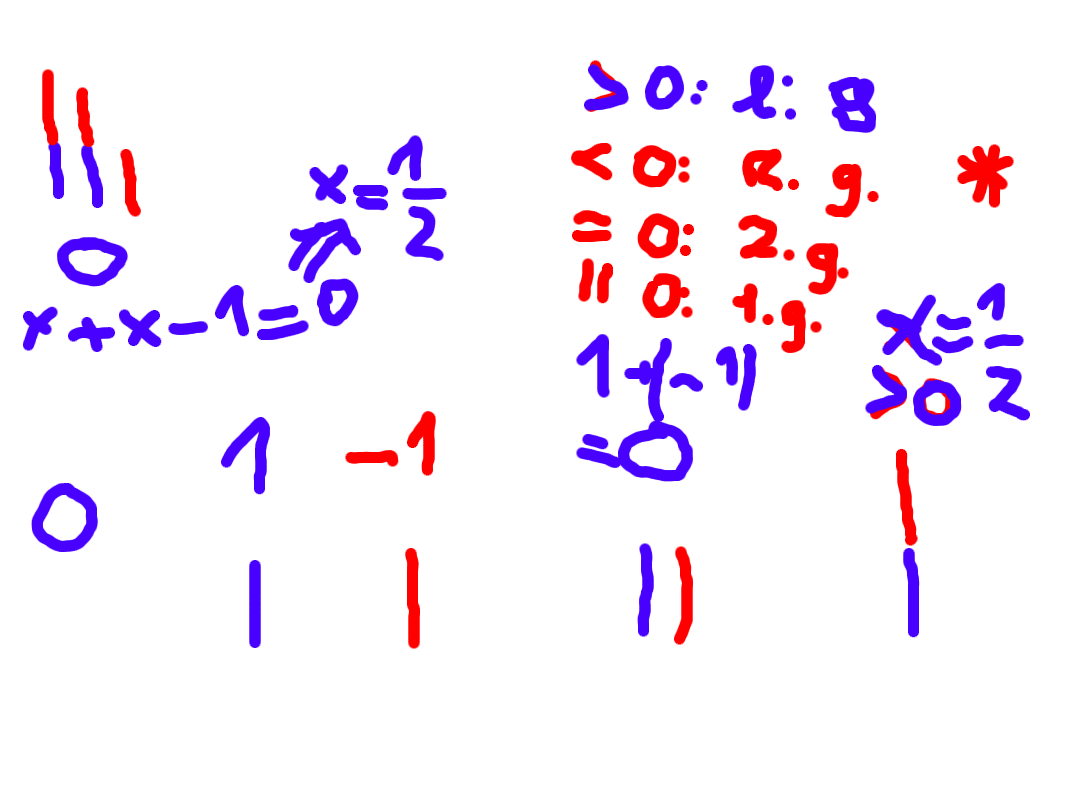
\includegraphics[width=\textwidth]{images/surreal2}}
\frame[plain]{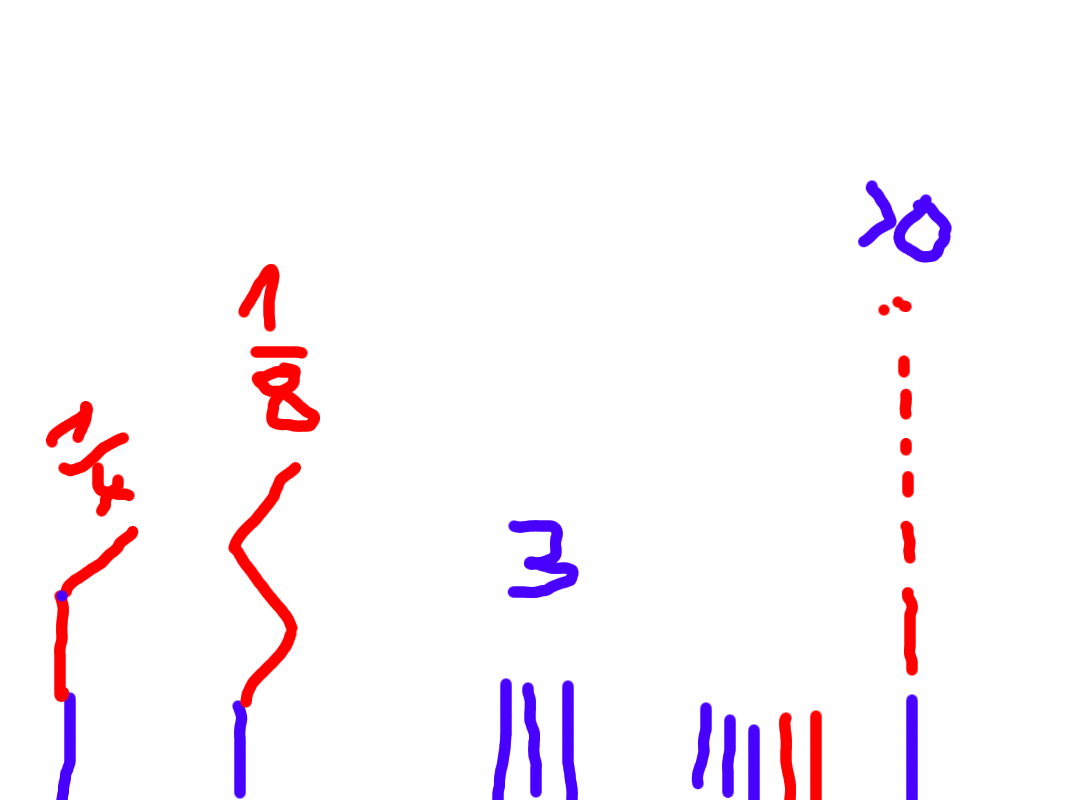
\includegraphics[width=\textwidth]{images/surreal3}}
\frame[plain]{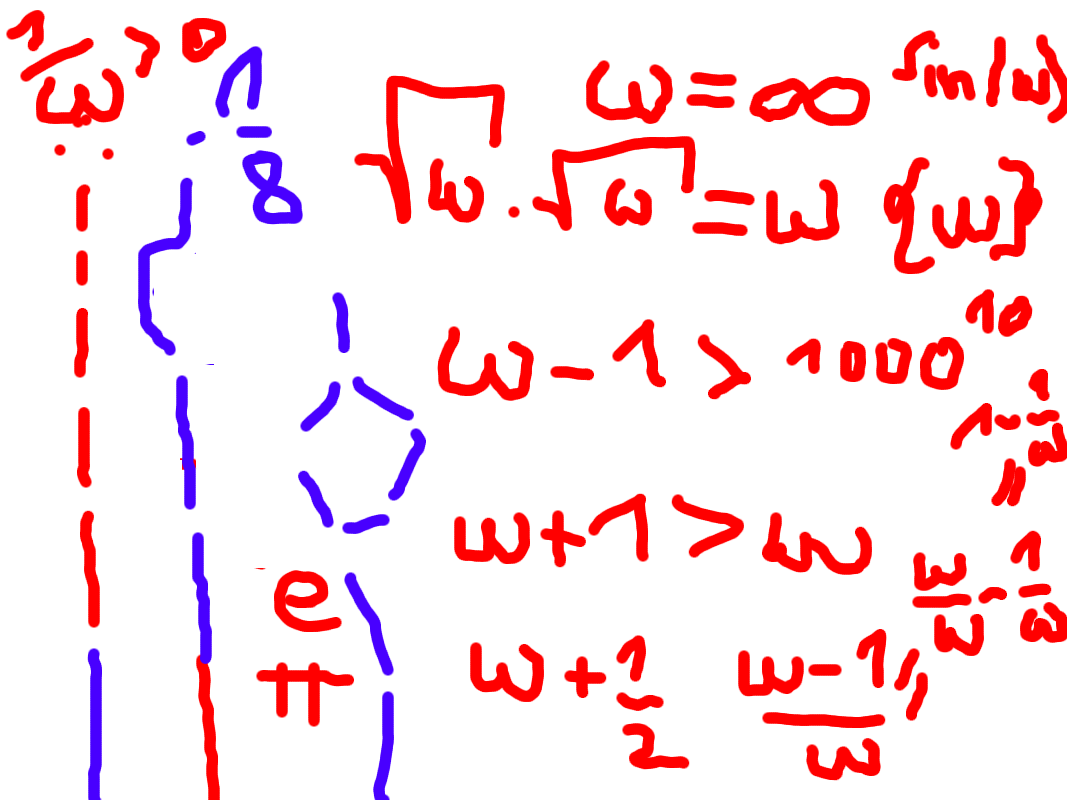
\includegraphics[width=\textwidth]{images/surreal4}}

\frame[plain]{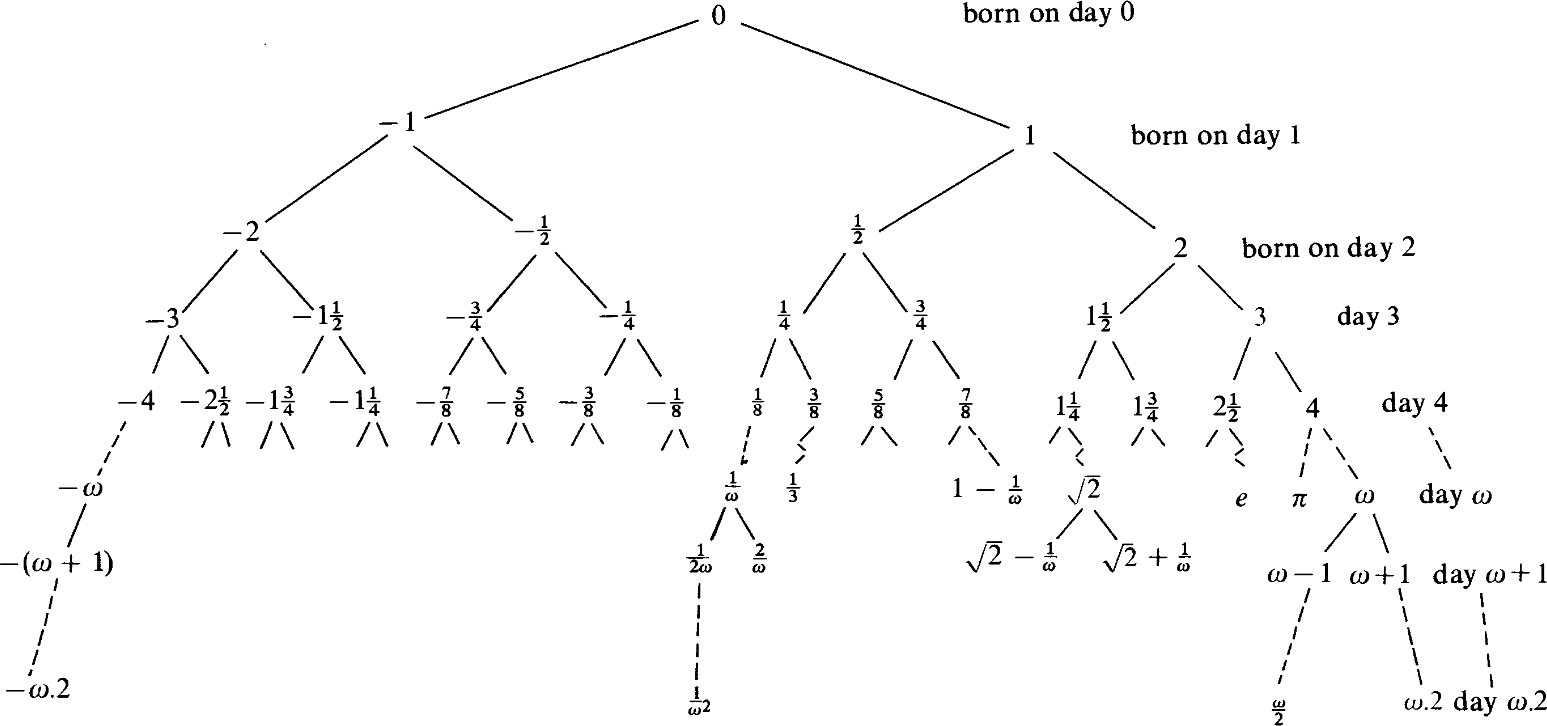
\includegraphics[width=\textwidth]{images/stammbaum-der-surrealen-zahlen}}

\frame[plain]{\footnotesize\justifying
  Tolle verständliche Quellen für surreale Zahlen und Games sind:
  \begin{itemize}
  \item \href{https://en.wikipedia.org/wiki/Surreal_number}{Wikipedia. Surreal
  numbers.}
  \item
  \href{https://web.archive.org/web/20151121050005/http://www.tondering.dk/download/sur16.pdf}{Claus
  Tøndering. Surreal numbers -- an introduction.}
  \item
  \href{http://scienceblogs.com/goodmath/2006/08/17/introducing-the-surreal-number/}{Good
  Math, Bad Math. Introducing the surreal numbers.}
  \item Die drei aufgeführten Bücher.
  \end{itemize}
  Diese Literatur setzt keine Vorkenntnisse aus einem Mathe-Studium voraus! Sie
  ist also auch für euch, liebe Schülerinnen und Schüler, geeignet. Außerdem
  gibt es eine Mischung aus Erklärung und Aufgabensammlung:
  \begin{itemize}
  \item
  \href{http://rawgit.com/iblech/mathezirkel-kurs/master/thema02-surreale-zahlen/blatt02.pdf}{Matheschülerzirkel
  Augsburg. Surreale Zahlen.}
  \end{itemize}

  \hfill
  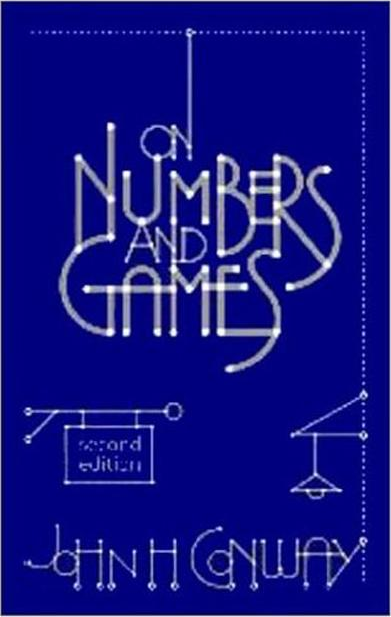
\includegraphics[height=0.4\textheight]{images/book-onag}
  \hfill
  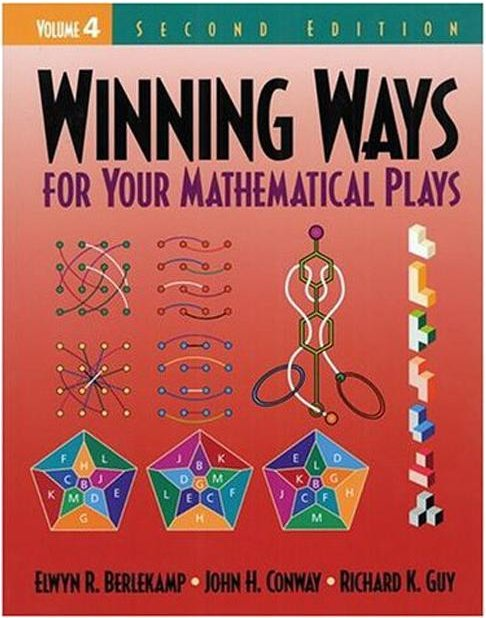
\includegraphics[height=0.4\textheight]{images/book-winning-ways}
  \hfill
  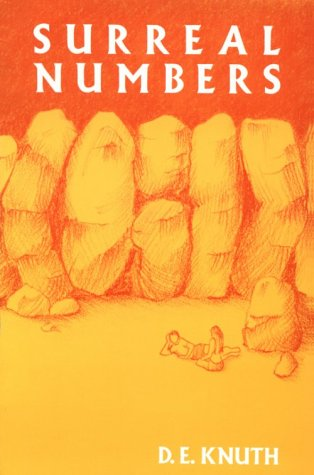
\includegraphics[height=0.4\textheight]{images/book-knuth}
  \hfill{}{}
}

\end{document}
